\chapter{Estado del Arte}

\section{Convertidores de Potencia}

\section{Semiconductores}



\subsection{Transistor MOSFET}

Un transistor de efecto de campo semiconductor de óxido de óxido metálico o MOSFET es un tipo especial de transistor que funciona como un interruptor o una puerta para la electricidad.Puede activar o desactivar el flujo de corriente utilizando un pequeño voltaje.MOSFET tiene tres partes principales: la puerta, el drenaje y la fuente.

MOSFET utiliza un pequeño voltaje en la puerta para controlar el flujo de corriente.A diferencia de otros interruptores, usa muy poca potencia.Esto lo hace rápido, eficiente y perfecto para circuitos donde el ahorro de energía es importante.Encontrará MOSFET en casi todas partes en la electrónica moderna porque son pequeños, confiables y hacen el trabajo en silencio detrás de escena.

Este trabajo se ha centrado especialmente en los , los llamados transistores de efecto campo metal-óxido-semiconductor (MOSFET).

Un MOSFET funciona usando voltaje en la puerta para controlar el flujo de corriente entre la fuente y el drenaje.Cuando aplica voltaje a la puerta, afecta el área debajo del semiconductor.Este cambio permite o bloquea el flujo de corriente a través del dispositivo.

En MOSFET de canal N, un voltaje positivo en la puerta crea una ruta para que los electrones se muevan, lo que permite que la corriente fluya.Cuanto más voltaje aplique, más fácil es que la corriente pase.

En el canal P MOSFET, el proceso se invierte.Aplica un voltaje negativo para permitir el flujo de corriente atrayendo cargas positivas (agujeros).

En ambos tipos, la puerta actúa como una señal de control: no permite que la corriente fluya en ella, sino que influye en si la corriente puede moverse a través del dispositivo.Esto hace que el MOSFET sea eficiente y rápido para cambiar en circuitos electrónicos.

Cuenta con tres terminales, llamados drenador (D), fuente (S) y puerta (G)

\begin{figure}
    \label{figure: Esquema MOSFET}
    \centering
    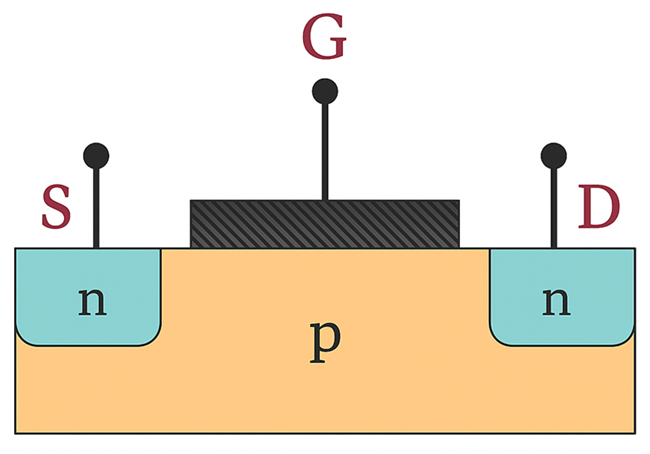
\includegraphics[width = 0.5  \textwidth]{Imagenes/MOSFET Canal N Esquema.png}
    \caption{Estructura MOSFET de canal N \cite{MOSFET_esquema}}
\end{figure}

